

\documentclass[11pt]{article}
\usepackage[utf8]{inputenc}
\usepackage{geometry}
\usepackage{graphicx}
\usepackage{hyperref}
\usepackage{amsmath}
\usepackage{listings}
\usepackage{xcolor}
\usepackage{float}
\usepackage{subcaption}
\usepackage{algorithm}
\usepackage{algpseudocode}
\usepackage{booktabs} % For prettier tables
\usepackage{siunitx}
\usepackage{amssymb}
\usepackage{subcaption}

% Set page margins
\geometry{a4paper, margin=1in}

% Set up code listing style
\lstset{
    basicstyle=\ttfamily,
    commentstyle=\color{gray},
    keywordstyle=\color{blue},
    stringstyle=\color{red},
    showstringspaces=false,
    captionpos=b
}

\title{Discovering Symbolic Models from Deep Learning
with Inductive Biases: Reproduction Report}
\author{Vishal Jain}
\date{\today}

\begin{document}
\section{Introduction}
% Introduce what this report is tackling: reproducing subset of results from Cranmer et al.

% Why is the problem important: Motivate why even bother to develop a framework that approximates nns with symbolic models.

% How are we going to do it: High level overview of the approach taken in the report.

% Background: 
% New concepts - symbollic regression, graph neural networks. Inductive biases.



% What is the report about
The aim of this report is to reproduce the key results of the paper \textit{Discovering Symbolic Models from Deep Learning with Inductive Biases} by \textit{Cranmer et al.}. The main contributions of the paper are two fold - first the presentation of a systematic framework whereby inductive biases can be employed to distill low dimensional symbolic approximations to learned neural networks. The second is showing its successful application of the framework in 3 contexts: rediscovering force laws, rediscovering Hamiltonians and discovering a new equation for a nontrivial cosmology problem. Since the time of the paper's publication, there have been several successful applications of the framework to a variety of problems more complex than the ones presented in the paper (cite some examples).
% What are subset are we exploring 
The scope of this report is limited to the reproducibility of the experiments relating to the rediscovery of force laws. However, in doing so, the wider contribution of the framework will be validated.
% Why.
\subsection{Motivation}
First the motivation behind symbolic distillation is explored. Why would it be desirable to approximate a high dimensional neural network with a low dimensional symbolic model? The answer lies in the scientific method itself and the unreasonable effectiveness of mathematics in the natural sciences.
When using neural networks as a tool for science, the lack of interpretability is a major drawback. Science is not just about making predictions, but also about understanding the underlying mechanisms that govern the phenomena being studied. Neural networks are famously known to be black boxes, with the decision-making process being opaque to the user. If they are to be used for science, there needs to be some distillation of what the network has learned in a form that is interpretable to humans. 
Symbolic models are a natural choice for this task, as they provide a compact and interpretable representation of the underlying mechanisms due to their low dimensionality. Further, they are likely to generalise better to out of distribution data than the neural network itself, indeed in the findings of the paper, the symbolic models generalised better than the neural networks to unseen data. This is due to the unreasonable effectiveness of mathematics in the natural sciences, for whatever reason, choosing to describe the world in terms of closed form low dimensional mathematical equations has been shown to be a very good inductive bias. 

\subsection{Inductive Biases}
It is important to fully explore the concept of effective inductive biases. Inductive biases can be understood as the priors that a set of modelling assumptions impose on the space of possible functions. To illustrate the challenges neural networks face in scientific modelling, consider an experiment depicted in Figure \ref{fig:nn_vs_sym_sin} where a neural network, consisting of a single layer with 100 ReLU activations, is trained on data points sampled from a sinusoidal function. While this high-dimensional neural network fits the training data adequately, it struggles to generalise. Conversely, one can searching for an analytic equation using a technique known as symbollic regression. Symbolic regression is a supervised machine learning method that constructs analytic functions to model data. Applying symbolic regression to the same dataset yields the equation $y = sin(x)$, which perfectly describes the data. Thus, applying the inductive bias that the underlying function is a closed form low dimensional equation, results in a model that generalises, in this case, perfectly. This example highlights the advantages of analytic equations, which not only require far fewer parameters than neural networks to represent, but also lead to more reliable generalisation to out-of-distribution data. 

\begin{figure}[H]
    \centering
    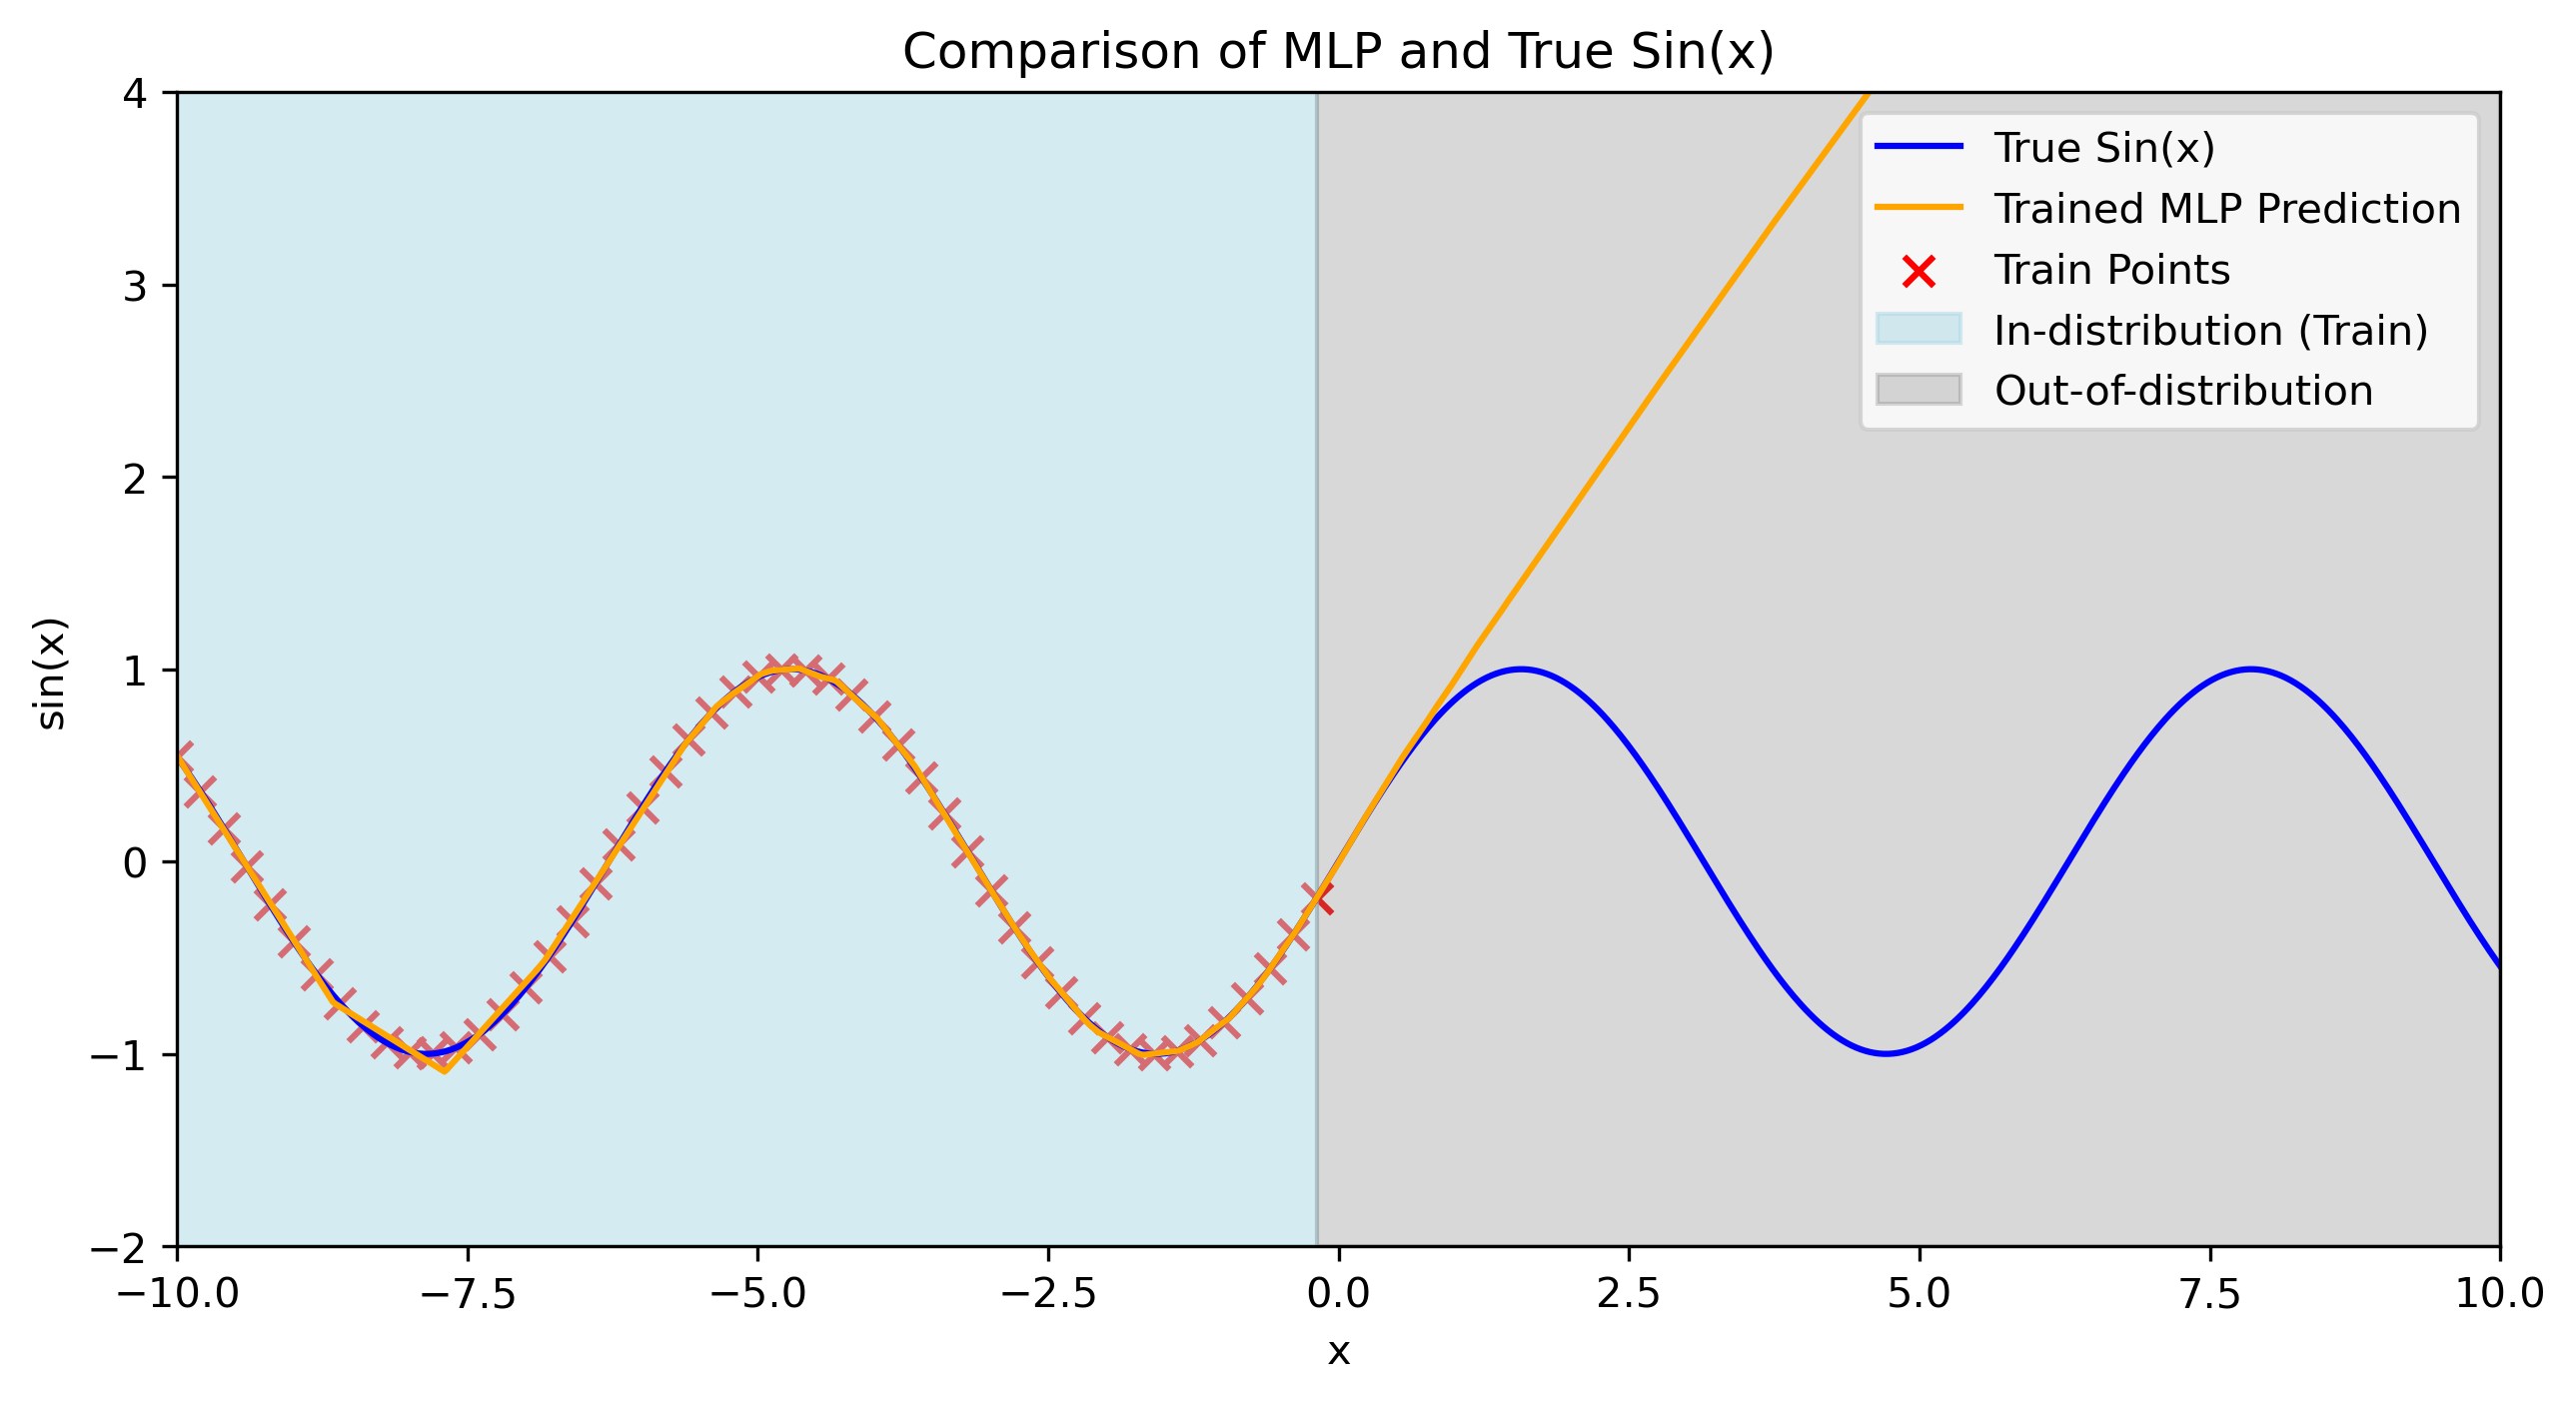
\includegraphics[width=0.9\textwidth]{figs/analytic_vs_nn_inductive_bias.png}
    \caption{Neural network prediction (one layer network with width 100 and ReLU activations)  versus symbolic model for sinusoidal dataset. The symbolic model is $y = sin(x)$.}
    \label{fig:nn_vs_sym_sin}
\end{figure}

\subsection{Symbolic Distillation Framework}
The general framework prescribed by the paper for symbolic distillation is as follows:
\begin{itemize}
    \item Design a neural network with an architecture that has a seperable internal structure and an inductive bias that is well suited to modelling the underlying problem.
    \item Train the model with regularisation techniques that encourage the network to learn a low-dimensional representation of the data.
    \item Replace a component of the neural network with a symbolic model that approximates the neural network's output.
    \item Retrain the neural network with the symbolic model as a component, and repeat the process until all components of the neural network have been replaced with low dimensional symbolic models.
\end{itemize}

% Why even add NNs - factorisation of the search space.
This framework may prompt the question: what is the necessity of employing neural networks initially? Why not directly utilize symbolic regression? The issue arises from the high dimensionality of modern datasets, which renders the application of symbolic regression, essentially a brute-force search over the space of all possible equations, computationally infeasible. To illustrate this point and the motivation behind this work, consider the problem of discovering a force law from a dataset of observed instantaneous accelerations of particles $\mathbf{a}_i \in \mathbb{R}^n$ and their positions $\mathbf{x}_i \in \mathbb{R}^n$. Assume a force law of the form $\mathbf{f}_{ij} = -k |\mathbf{x}_i - \mathbf{x}_j|$, with $\mathbf{a}_i = \frac{\mathbf{F}_i}{m_i}$, where $\mathbf{F}_i = \sum_j \mathbf{f}_{ij}$. To learn symbolic models for the acceleration $\textbf{p}(\textbf{x})$ and the pairwise force $\textbf{q}(\textbf{x})$, one can apply the inductive bias $\textbf{a}_i = \textbf{p}(\sum_j \textbf{q}(\textbf{x}_i, \textbf{x}_j))$. If the symbolic regression model needs to search $N$ equations to fit a given model, the search space scales as $O(N^2)$. However, if neural networks are first used to approximate the functions $\mathbf{p}(x)$ and $\mathbf{q}(x)$, and symbolic regression is subsequently applied to approximate these neural networks, the models can now be fit independently, reducing the search space to $O(N)$. If the dimensionality of the problem $n$ increases or the force law becomes more complex, the number of equations $N$ required to search also increases significantly. Therefore, this factorization of the search space is essential to make symbolic regression tractable for high-dimensional problems.
\subsection{Graph Neural Networks}
The work in the original paper and this report is primarily related to the class of problems which can be classed as interacting particle problems. This type of problem describes a very broad range of most problems encountered in physics. The graph neural network architecture applies a well suited inductive bias to these problems. This section will briefly describe the fundamental components of the graph neural network architecture and why it is well suited to interacting particle problems.

A graph neural network (GNN) is a specialised architecture designed to operate on graph data structures, where nodes represent particles and edges represent pairwise interactions between particles. In this context, each node has an associated feature vector encoding properties such as position, velocity, mass, and charge. The GNN operates through a scheme of message passing, involving two main components: the edge model ($\phi_e$) and the node model ($\phi_v$).
\paragraph*{Edge Model ($\phi_e$):}
   \begin{itemize}
       \item The edge model is applied to each edge in the graph.
       \item It takes as input the feature vectors of the two nodes connected by the edge.
       \item Formally, $\phi_e : \mathbb{R}^{d_v} \times \mathbb{R}^{d_v} \rightarrow \mathbb{R}^{d_e}$, where $d_v$ is the dimensionality of the node feature vectors, and $d_e$ is the dimensionality of the edge messages.
       \item The output of the edge model is called an edge message.
   \end{itemize}

\paragraph*{Node Model ($\phi_v$):}
   \begin{itemize}
       \item Once every edge has an associated edge message, the node model is applied to each node in the graph.
       \item It takes as input the feature vector of the node and the aggregated edge messages from all inbound edges.
       \item Aggregation is performed using a summation operator.
       \item Formally, $\phi_v : \mathbb{R}^{d_v} \times \mathbb{R}^{d_e} \rightarrow \mathbb{R}^{d_v'}$, where $d_v'$ is the dimensionality of the updated node feature vectors.
       \item The output of the node model is the updated node feature vector.
   \end{itemize}

This message-passing process is repeated for a number of layers, with the output of the final layer being the output of the graph neural network. The computational graph of the GNN is shown in Figure \ref{fig:gnn}, illustrating the interactions between nodes and edges through the edge and node models.

The graph neural network is an appropriate inductive bias for a variety of reason. Firstly, many important forces in physics are defined on pairs of particles, analogous to the message function of the Graph Networks. Further, the summation that aggregates messages is analogous to the calculation of the net force on a receiving particle. Finally, the node function is analogous to the application of Newton's second law: acceleration equals the net force (the summed message) divided by the mass of the receiving particle. Further, the graph neural network architecture is invariant under particle permutations, which is a desirable property for a model which represents interacting particle problems. 

It will be the edge and node models of the graph neural network that will be replaced by symbolic models in the symbolic distillation framework. The goal will be to recover the underlying force law used to generate the data.
\begin{figure}[H]
    \centering
    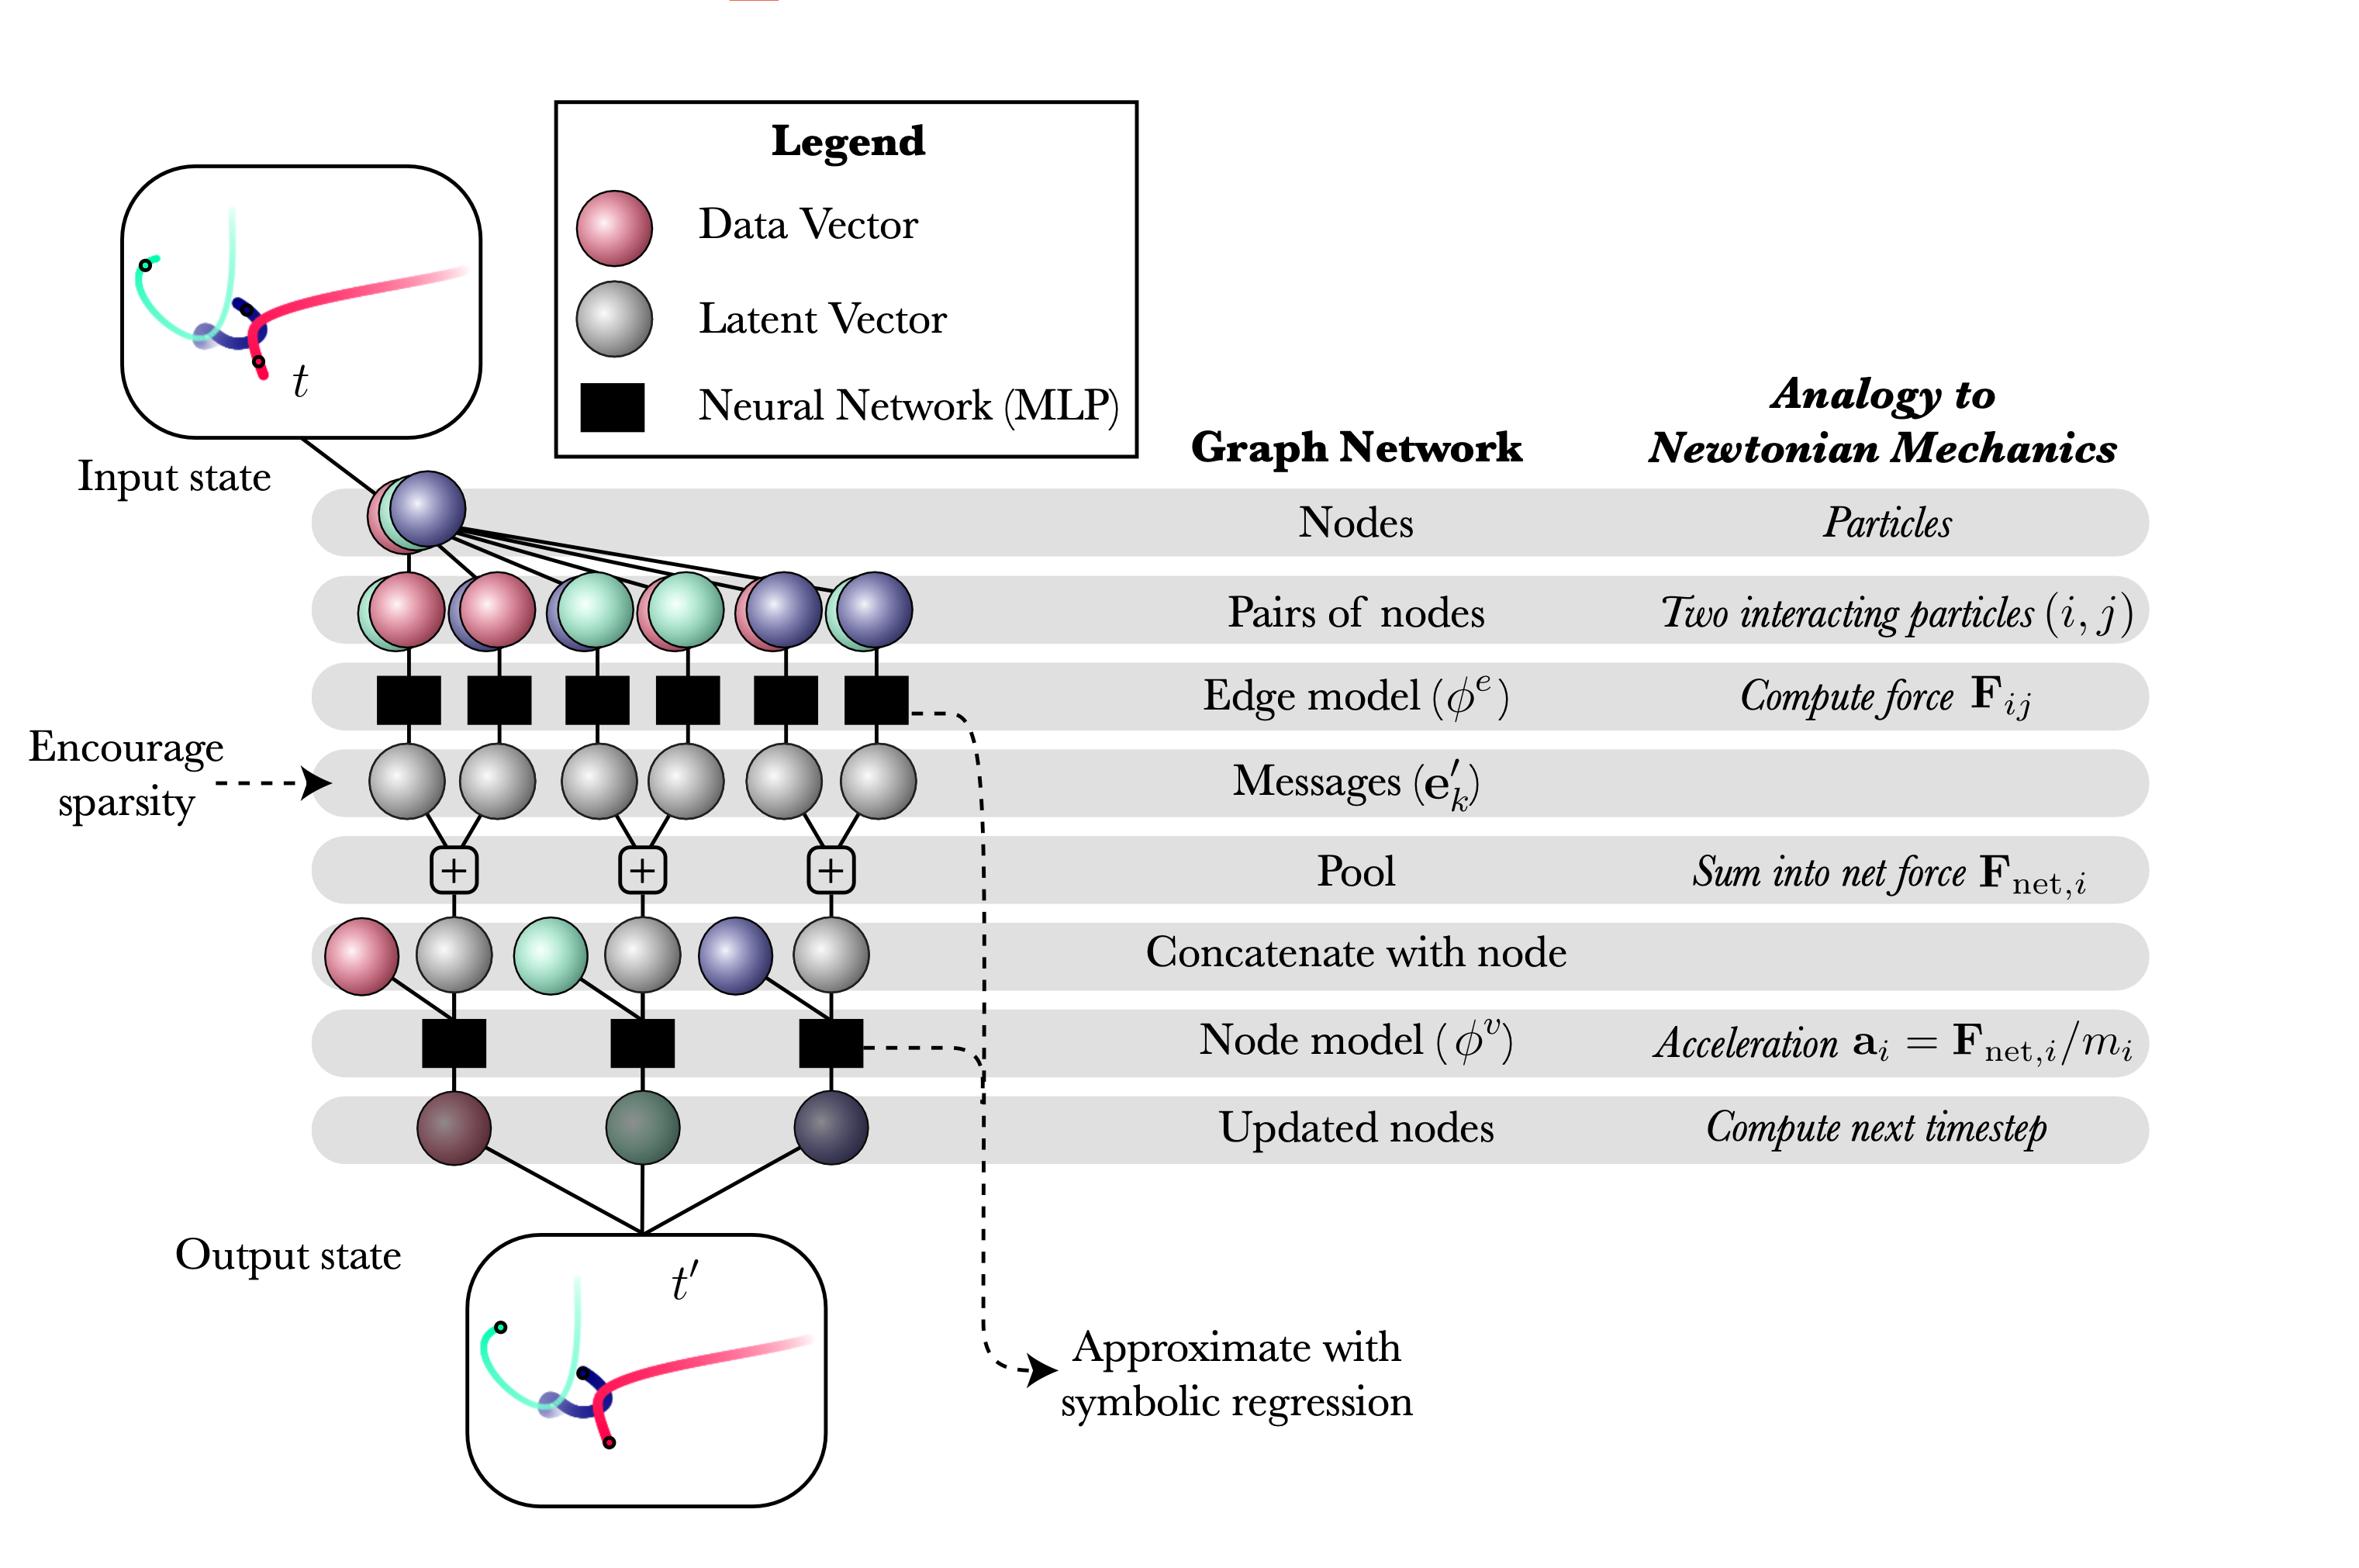
\includegraphics[width=0.9\textwidth]{figs/gnn_diagram.png}
    \caption{Computational graph of the graph neural network architecture. Diagram taken from Cranmer et al. \cite{cranmer2020discovering}}
    \label{fig:gnn}
\end{figure}
% Explain what they are and why they present the appropriate inductive bias for the problem.

% force law interacting particle problems - Fri
% Introduce the data briefly and the pipeline for the problem.
\section{Data}
This section will outline the datasets used in the experiments and the pipeline for the problem. The dataset consists of N-body particle simulations for a variety of force laws. From the original paper, the following force laws are investigated:
\begin{itemize}
    \item Spring: \(\textbf{f}_{ij} = -(|\textbf{r}_{ij} - 1|) \hat{\textbf{r}}_{ij}\)
    \item \(\frac{1}{r}\) Orbital force: \(\textbf{f}_{ij} = -\frac{m_i m_j\hat{\textbf{r}}_{ij}}{|\textbf{r}_{ij}|}\)
    \item \(\frac{1}{r^2}\) Orbital force: \(\textbf{f}_{ij} = -\frac{m_i m_j \hat{\textbf{r}}_{ij}}{|\textbf{r}_{ij}|^2}\)
    \item Charge: \(\textbf{f}_{ij} = -\frac{q_i q_j \hat{\textbf{r}}_{ij}}{|\textbf{r}_{ij}|^2}\)
\end{itemize}
Each force law was simulated in 2D and 3D, with 4 and 8 particles respectively. For each experiment, 10000 simulations were run in parallel for 500 time steps. This was split 3:1 to obtain the training and validation set. The test set was generated separately. The initial positions and velocities were randomly sampled from a normal distribution, the mass was sampled from a log normal distribution and the charge was drawn randomly from the set \(\{-1, 1\}\). 
% Original paper dataset size vs this one 
It is worth noting that the original paper ran each simulation for 1000 time steps, however, to avoid model training times becoming prohibitively long, the simulations were run for half the number of time steps. The step size varies for each simulation due to the differences in scale. It is: 0.005 for \( \frac{1}{r} \), 0.001 for \( \frac{1}{r^2} \), 0.01 for Spring, 0.001 for Charge. The code used to generate the simulations is available in the repository under the \texttt{simulations} directory. 
% Preprocessing
\subsection{Preprocessing}
Due to the nature of orbital and charge force laws, their dependence on \(r\) with a negative power can lead to exploding force values when particles are too close. This causes the data to vary over a scale too large for a neural network to learn effectively. To mitigate this, a small epsilon (\(10^{-2}\)) was added to the denominator, squashing \(r\) values into a more manageable range. Despite this, some experiments were found to have velocity distributions that still contaned extremely large outliers. To address this, a preprocessing step was introduced. The velocities and accelerations were pruned based on upper and lower percentile bounds. If any particle in a given timestep had a velocity or acceleration outside these bounds, the entire graph for that timestep was removed. This ensured that only timesteps where all particles had acceptable values were retained, improving data quality and consistency. Note, while this breaks the time continuity of the data, it is important to note that the data need not be continuous in time, as each time step defines a complete graph input to the neural network. The impact of this preprocessing step for the 2D Charge data in \ref{fig:distributions}. To see more detailed summary statistics showing the effect of this step, refer to the appendix.
\begin{figure}[H]
    \centering
    \begin{subfigure}{0.9\textwidth}
        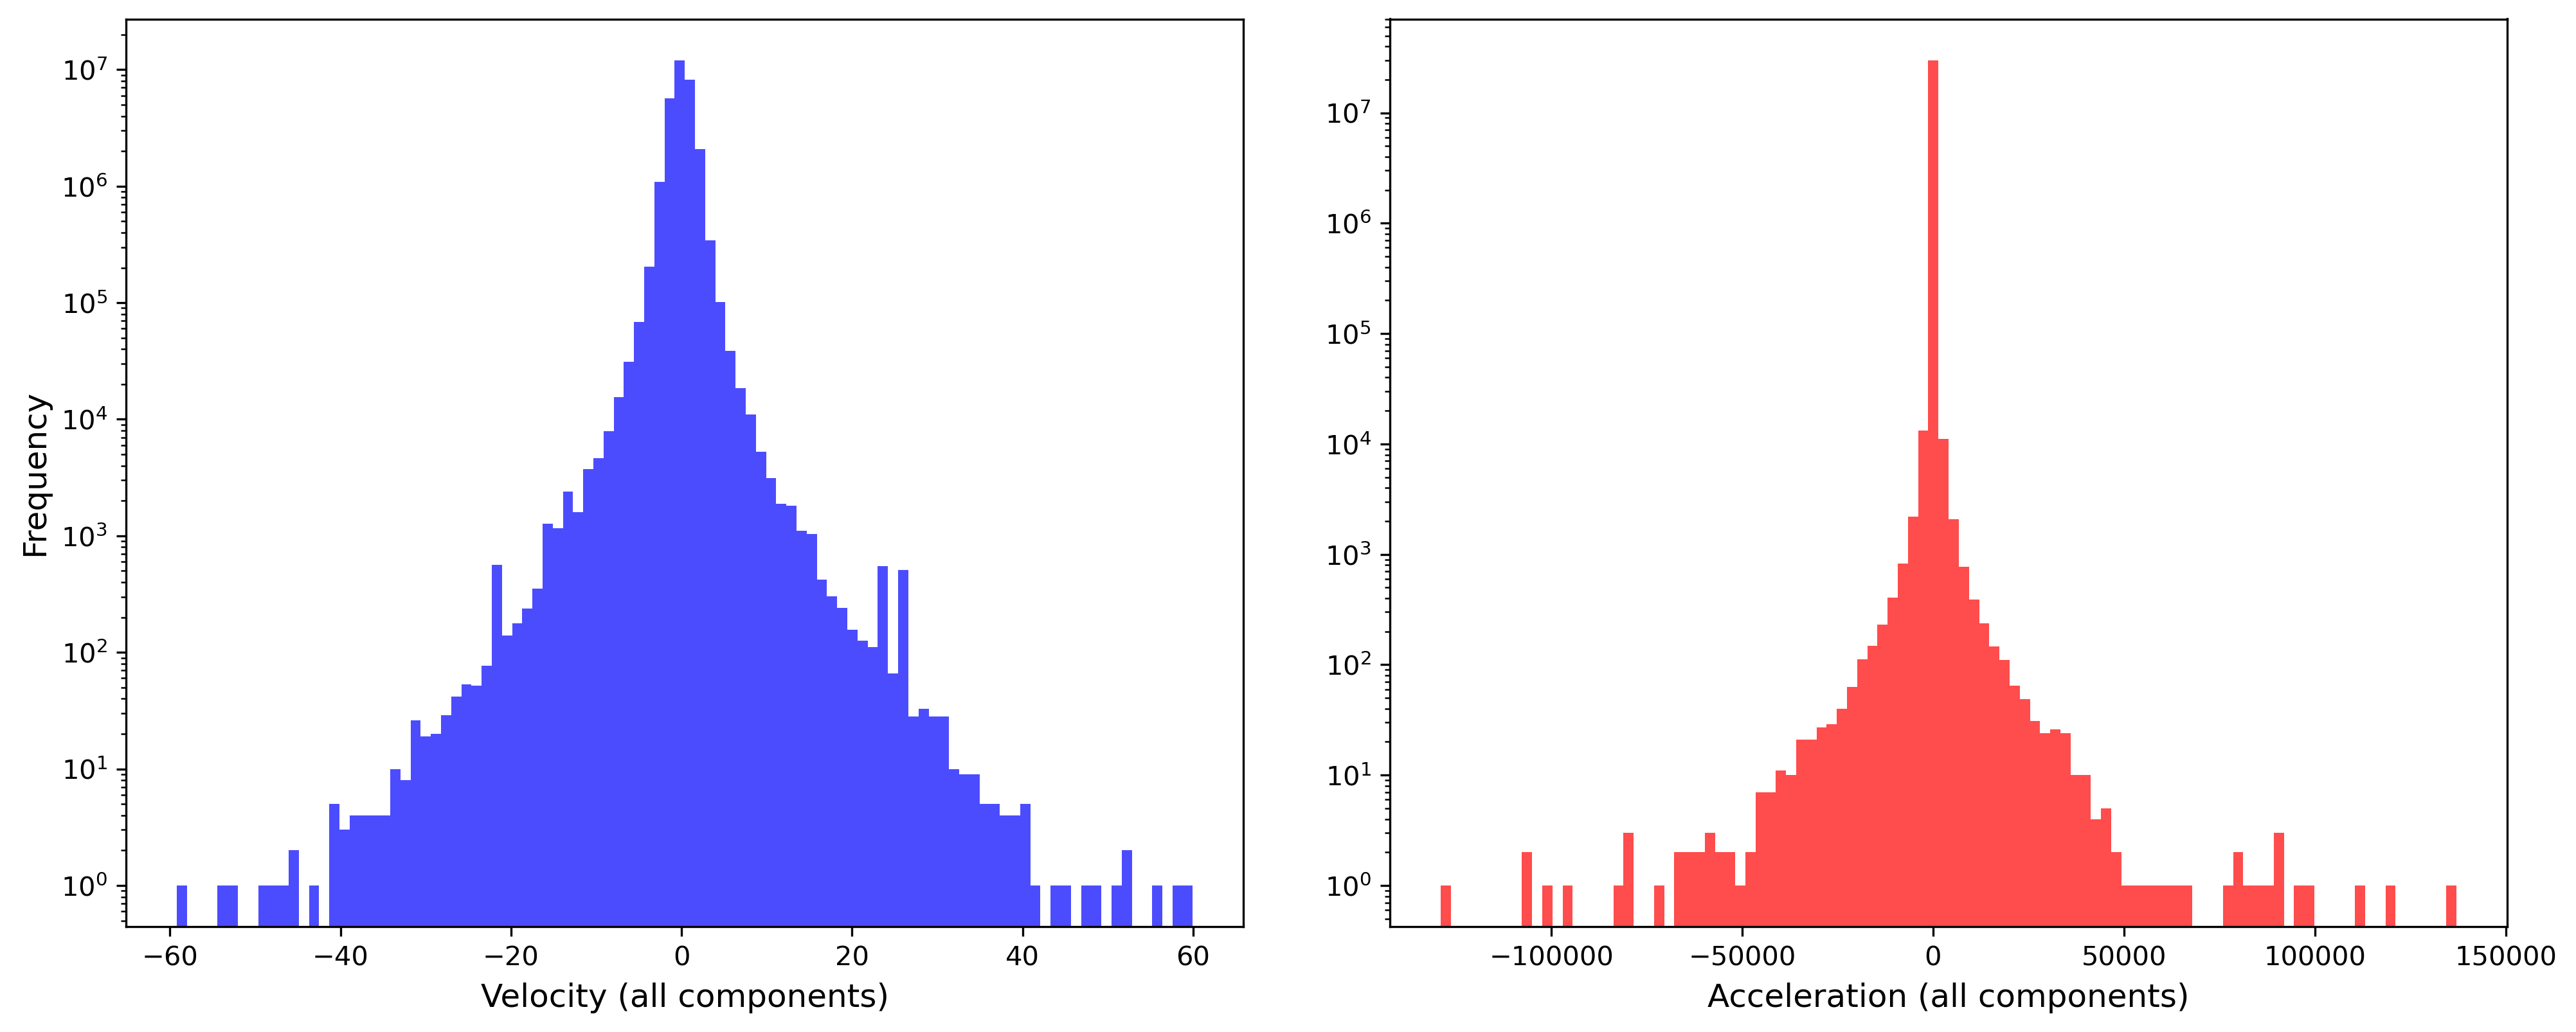
\includegraphics[width=\textwidth]{figs/charge_2_accel_vel_dist_unpruned.png}
        \caption{Charge 2D velocity distribution}
        \label{fig:charge_2_vel_dist_unpruned}
    \end{subfigure}
    \begin{subfigure}{0.9\textwidth}
        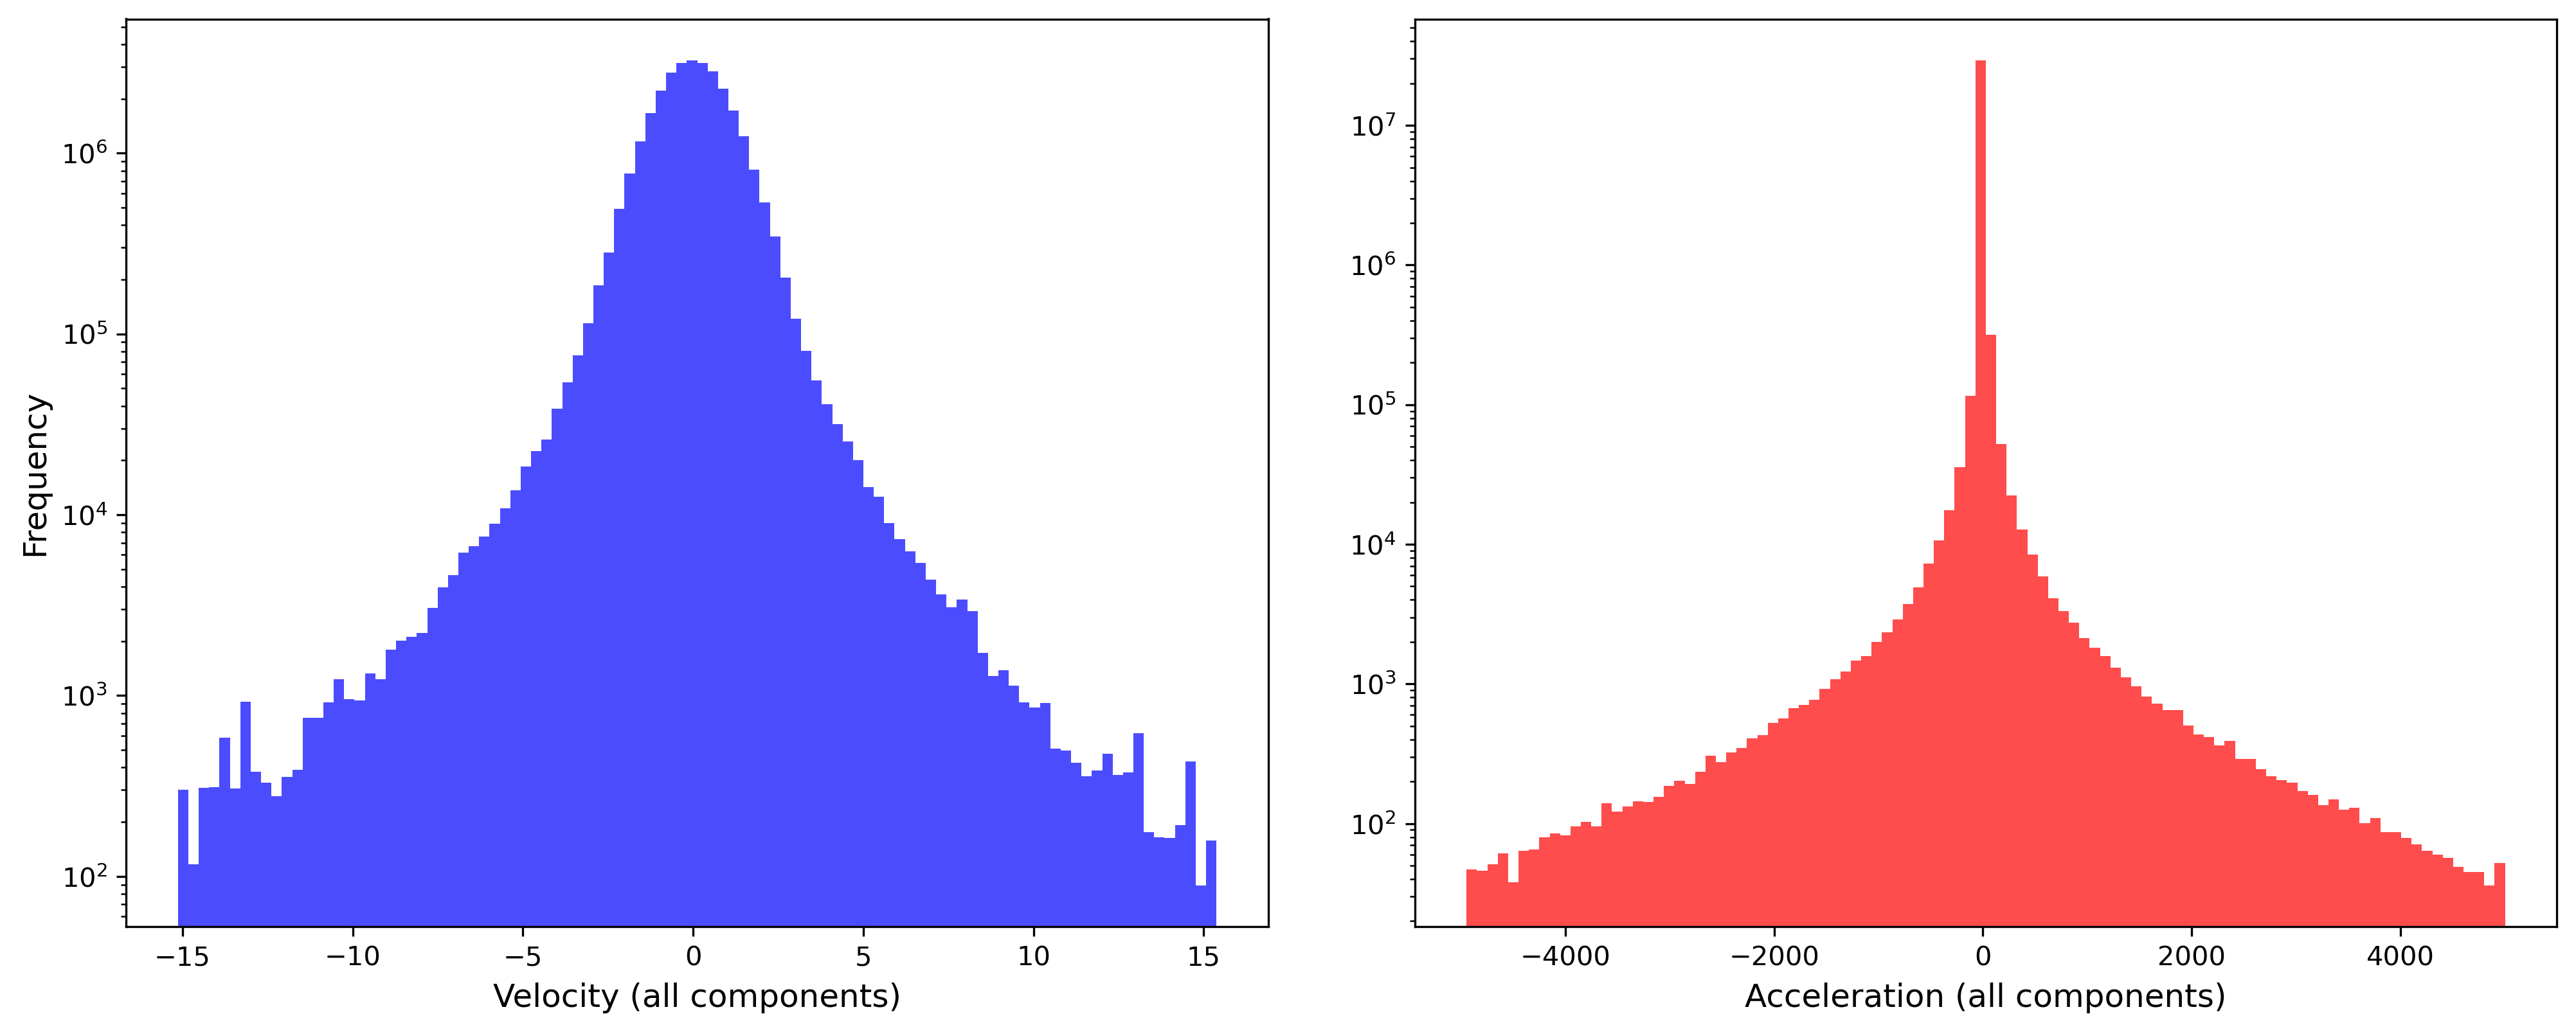
\includegraphics[width=\textwidth]{figs/charge_2_accel_vel_dist_pruned.png}
        \caption{Charge 2D velocity distribution (pruned)}
        \label{fig:charge_2_vel_dist_pruned}
    \end{subfigure}
    \caption{Velocity and acceleration distributions for Charge 2D data before and after preprocessing}
    \label{fig:distributions}
\end{figure}


\section{Method}
This section outlines the method used to train a graph neural network to predict instantaneous accelerations of particles.

\subsection{Training strategies}
This report investigates 4 of the training strategies outlined in the original paper. The training strategies are as follows: standard, KL, bottleneck and L1. 

\paragraph*{Standard Strategy}
The standard training strategy serves as the baseline case where the edge message dimensionality is 100 and the loss does not include any regularisation terms. Here the loss function is given by the mean absolute error between the predicted and true accelerations.

\paragraph*{KL Strategy}
The KL strategy involves sampling edge messages from a multivariate normal distribution as defined by the output of the edge model, which is now a 200-dimensional vector, with the first 100 dimensions representing the mean and the second 100 dimensions representing the log variance. Additionally, the average Kullback-Leibler divergence penalty over all edge messages, using a standard normal as the prior, is added to the loss. The weight of this term is set to \(1.0 \).

\paragraph*{L1 Strategy}
The L1 strategy is the same as the standard, except it now incorporates the L1 norm of the edge message as a regularisation term, averaged over all edge messages, in the loss. The weight of this term is set to \(1.0 \times 10^{-2}\).

\paragraph*{Bottleneck Strategy}
The bottleneck strategy is the same as the standard, however now aligns the dimensionality of the edge message with the dimensionality of the problem (2 or 3).

% Introduce the architecture of the model
\subsection{Model Architecture}
The architecture of the graph neural network (GNN) employed across various training strategies is consistent, except for variations in the output dimension of the edge model. The GNN comprises two multi-layer perceptrons (MLPs): the edge model and the node model.

\paragraph*{Edge Model} This model consists of two hidden layers, each with 300 units and ReLU activation functions. It takes as input the concatenated feature vectors from a pair of nodes connected by an edge in the graph. Each input vector is a $(2d+2)$-dimensional representation of position, velocity, mass, and charge, where $d$ represents the problem's dimensionality (2 or 3). The output dimension of the edge model varies depending on the training strategy.

\paragraph*{Node Model} Mirroring the edge model in structure, the node model takes as input the summed edge messages from all inbound edges to a given node, concatenated with the node's feature vector. Its output is a vector of dimension 2 or 3, corresponding to the predicted instantaneous acceleration of the node.

\subsection{Model Training}
The network is trained over 100 epochs using the Adam optimizer with an initial learning rate of \(0.001\) and weight decay set to \(1.0 \times 10^{-8}\). It is worth noting that this is half the number of epochs used in the original paper. The learning rate is modulated by the 1cycle learning rate policy \cite{smith2018superconvergence}, which increases the learning rate to a peak of \(0.001\) before gradually decreasing it by a factor of \(100,000\), adhering to a pre-defined schedule. Random translation is used as a form of data augmentation to improve the model's generalisation capabilities. The model is trained on a single NVIDIA A100 GPU.

\subsection{Symbolic Regression of the Network}
% Explain how the sybolic regressor was fit - used less operations than the paper to make it easier to reduce the search space
After training the model end to end, the edge and node model are symbolically distilled using the \texttt{PySR} package \cite{cranmer2023interpretable}. PySR's internal search algorithm is a multi-population evolutionary algorithm, which consists of a unique evolve-simplify-optimise loop, designed for optimisation of unknown scalar constants in newly-discovered empirical expressions. The operators considered in the fitting process are $ +, -, \times , /$ as well as real constants. Note, this is a subset of the operators used in the original paper when fitting for symbolic models. This was done to reduce the search space and quickly check that the symbolic distillation framework was working as expected.

\subsubsection{Model Selection Criteria}
The best symbolic model is selected by evaluating the mean absolute error (MAE) and the complexity of the model. The complexity is scored by counting the number of occurrences of each operator, constant, and input variable. PySR outputs several equations at each complexity level. The chosen formula is one that maximises the fractional drop in MAE over an increase in complexity from the next best model.

\subsubsection{Symbolic Distillation of the Edge Model}
To symbolically distil the edge model, its inputs and outputs are recorded over the test set. The input comprises the concatenated feature vectors of two nodes connected by an edge, including the position, velocity, mass, and charge of each node ($(m_1, m_2, q_1, q_2, x_1, x_2, \ldots)$). Given that force laws depend on the relative positions of the nodes, To simplify, the positions are converted to $\Delta x = x_2 - x_1$ for displacement, similarly for $y$ (and $z$ in 3D), and $r = \sqrt{\Delta x^2 + \Delta y^2 + (\Delta z^2)}$ for distance. This array of $(m_1, m_2, q_1, q_2, \Delta x, \Delta y, (\Delta z), r)$ comprises as the input to the symbolic model. Next, the $d$ most significant components of the corresponding edge message are selected as the output labels for the symbolic regression model. Significance here is defined by the components of the edge message with the highest standard deviation across the samples, where $d$ is the dimensionality (2 or 3). In the bottleneck strategy, the edge message is already of the correct dimensionality, so no further processing is needed. 5000 such samples are collected from the data in the test set, and the symbolic model is fit to these data points.

\subsubsection{Symbolic Distillation of the Node Model}
The symbolic distillation of the node model is similar to that of the edge model. The input to the symbolic model is the node's feature vector, which includes the position, velocity, mass, and charge of the node ($(m_1, q_1, x_1, \ldots)$), and the aggregated inbound edge messages. The aggregation is not performed over the full 100 dimensions of the edge message, but rather the $d$ most significant components, where $d$ is the dimensionality of the problem (2 or 3). The output of the symbolic model is the predicted instantaneous acceleration of the node. The symbolic model is fit to 5000 samples from the test set.


\subsection{Evaluation metrics}
To evaluate model performance, the mean absolute error (MAE) between the predicted and true accelerations is calculated over the test set. This metric assesses the predictive capabilities of the trained model. Additionally, the standard deviation of the top 15 edge messages is computed to evaluate the compactness of the learnt representations. This metric indicates whether the training resulted in a model that correctly captured the problem's dimensionality. The $R^2$ metric between the significant edge message components and a linear transformation of the true pairwise force is also calculated. The appendix of the original paper provides a mathematical argument for why the model would learn a linear transformation of the pairwise force. Furthermore, a qualitative binary classification of the models is conducted, considering a model successful if it can recover the correct force law. This is determined by comparing the symbolic model to the true force law and verifying if the symbolic model represents a linear transformation of the true force law.

\section{Implementation}

\section{Results}

% Code base structure, data storage, seed, local environment differences.
% Flowchart / graph.

\section{Reproducibility}
% Perhaps not just using the best model but checking if a slightly worse symbolic model was better.
% Talk about perhaps the more sensible thing would be to distill one at a time in accordance with the framework.
% Effect of training for fewer epochs
% Discuss challenges reproducing the results of the paper.
% Discuss how the code base is designed to give reproduible results
% Dataset storage.
% Dataset seed and local environment differences.
% Try to generate the dataset from a docker container to standardise the environment.
% Config files git commits, wandb
% Future work, squash velocity, use a larger eps and see if the model can learn this, squash the log var. For data pre processing 
% Preprocessing not in paper but got nans in kl otherwise
% Explore purely velocity based pre pru
% Adding more inductive biases eg newtons 3rd law and checking the results,

% Mon 
\section{Results}
\subsection{Pruned Test Set}
\begin{table}[h]
    \centering
    \begin{tabular}{lcccc}
    \hline
    Sim & KL & Standard & Bottleneck & L$_{1}$ \\
    \hline
    Spring 3d & 2.7227 & \textbf{0.0607} & 0.0640 & 0.0895 \\
    Charge 2d & nan & 1.1333 & \textbf{1.0220} & 1.1526 \\
    r$^{-1}$ 2d & 2.3468 & 0.0278 & \textbf{0.0263} & 0.0370 \\
    r$^{-2}$ 3d & 4.7287 & 0.7955 & \textbf{0.7664} & 0.8266 \\
    r$^{-2}$ 2d & 5.0257 & 0.9695 & \textbf{0.8214} & 0.8453 \\
    r$^{-1}$ 3d & 3.3449 & \textbf{0.0374} & 0.0376 & 0.0507 \\
    Spring 2d & 1.7688 & \textbf{0.0209} & \textbf{0.0209} & 0.0281 \\
    Charge 3d & 4.3491 & 0.5615 & \textbf{0.4956} & 0.5189 \\
    \hline
    \end{tabular}
    \caption{Performance statistics for Median}
    \label{tab:Median}
    \end{table}
    
    \begin{table}[h]
        \centering
        \begin{tabular}{lcccc}
        \hline
        Sim & KL & Standard & Bottleneck & L$_{1}$ \\
        \hline
        Spring 3d & 2.7299 & \textbf{0.0708} & 0.0753 & 0.1083 \\
        Charge 2d & nan & 3.0379 & \textbf{2.8888} & 3.0971 \\
        r$^{-1}$ 2d & 2.3706 & 0.0419 & \textbf{0.0397} & 0.0529 \\
        r$^{-2}$ 3d & 5.6837 & 1.7899 & \textbf{1.7301} & 1.7584 \\
        r$^{-2}$ 2d & 6.8925 & \textbf{2.8064} & 2.9481 & 2.8219 \\
        r$^{-1}$ 3d & 3.3496 & 0.0760 & 0.0763 & \textbf{0.0709} \\
        Spring 2d & 1.7579 & \textbf{0.0236} & 0.0267 & 0.0345 \\
        Charge 3d & 4.9074 & 1.1884 & \textbf{1.1209} & 1.1405 \\
        \hline
        \end{tabular}
        \caption{Performance statistics for Mean}
        \label{tab:Mean}
        \end{table}
        \begin{table}[h]
            \centering
            \begin{tabular}{lcccc}
            \hline
            Sim & KL & Standard & Bottleneck & L$_{1}$ \\
            \hline
            Spring 3d & 0.0808 & \textbf{0.0257} & 0.0282 & 0.0466 \\
            Charge 2d & nan & 5.2458 & \textbf{5.0082} & 5.1052 \\
            r$^{-1}$ 2d & 0.1610 & 0.0535 & \textbf{0.0527} & 0.0556 \\
            r$^{-2}$ 3d & 4.0685 & 2.6208 & 2.5762 & \textbf{2.5614} \\
            r$^{-2}$ 2d & 5.9032 & \textbf{5.2893} & 5.5942 & 5.5585 \\
            r$^{-1}$ 3d & 0.1447 & 0.1002 & 0.0965 & \textbf{0.0669} \\
            Spring 2d & 0.0682 & \textbf{0.0083} & 0.0133 & 0.0137 \\
            Charge 3d & 1.9053 & 1.7529 & 1.7078 & \textbf{1.7044} \\
            \hline
            \end{tabular}
            \caption{Performance statistics for Standard Deviation}
            \label{tab:Standard Deviation}
            \end{table}
            
\subsection{Pruned Test Set}
\begin{table}[h]
    \centering
    \begin{tabular}{lcccc}
    \hline
    Sim & KL & Standard & Bottleneck & L$_{1}$ \\
    \hline
    Spring 3d & 2.6960 & \textbf{0.0561} & 0.0589 & 0.0723 \\
    Charge 2d & 3.2076 & 0.4216 & \textbf{0.4178} & 0.4491 \\
    r$^{-1}$ 2d & 2.3171 & 0.0252 & \textbf{0.0236} & 0.0326 \\
    r$^{-2}$ 3d & 3.8290 & 0.1811 & \textbf{0.1806} & 0.2191 \\
    r$^{-2}$ 2d & 3.9970 & 0.559 & 0.4469 & \textbf{0.4419} \\
    r$^{-1}$ 3d & 3.2756 & 0.0281 & \textbf{0.0258} & 0.0405 \\
    Spring 2d & 1.7595 & 0.0197 & \textbf{0.0181} & 0.0248 \\
    Charge 3d & 3.3149 & \textbf{0.1062} & 0.1363 & 0.1544 \\
    \hline
    \end{tabular}
    \caption{Performance statistics for Median}
    \label{tab:Median}
    \end{table}

    \begin{table}[h]
        \centering
        \begin{tabular}{lcccc}
        \hline
        Sim & KL & Standard & Bottleneck & L$_{1}$ \\
        \hline
        Spring 3d & 2.6839 & \textbf{0.0566} & 0.0595 & 0.0728 \\
        Charge 2d & 3.2668 & 0.4662 & \textbf{0.4620} & 0.4829 \\
        r$^{-1}$ 2d & 2.3365 & 0.0254 & \textbf{0.0238} & 0.0326 \\
        r$^{-2}$ 3d & 3.8264 & 0.1753 & \textbf{0.1746} & 0.2128 \\
        r$^{-2}$ 2d & 4.0380 & 0.4745 & 0.4611 & \textbf{0.4499} \\
        r$^{-1}$ 3d & 3.2505 & 0.0283 & \textbf{0.0261} & 0.0408 \\
        Spring 2d & 1.7455 & 0.0200 & \textbf{0.0182} & 0.0249 \\
        Charge 3d & 3.3249 & \textbf{0.1095} & 0.1400 & 0.1574 \\
        \hline
        \end{tabular}
        \caption{Performance statistics for Mean}
        \label{tab:Mean}
        \end{table}
        
        \begin{table}[h]
            \centering
            \begin{tabular}{lcccc}
            \hline
            Sim & KL & Standard & Bottleneck & L$_{1}$ \\
            \hline
            Spring 3d & 0.0570 & \textbf{0.0031} & 0.0034 & 0.0038 \\
            Charge 2d & 0.4166 & 0.2107 & 0.1859 & \textbf{0.1783} \\
            r$^{-1}$ 2d & 0.1466 & 0.0048 & 0.0047 & \textbf{0.0040} \\
            r$^{-2}$ 3d & 0.2638 & \textbf{0.0418} & 0.0427 & 0.0497 \\
            r$^{-2}$ 2d & 0.5566 & 0.1688 & 0.1666 & \textbf{0.1420} \\
            r$^{-1}$ 3d & 0.1011 & \textbf{0.0028} & 0.0029 & 0.0037 \\
            Spring 2d & 0.0656 & \textbf{0.0013} & \textbf{0.0013} & 0.0015 \\
            Charge 3d & 0.1677 & \textbf{0.0153} & 0.0222 & 0.0189 \\
            \hline
            \end{tabular}
            \caption{Performance statistics for Standard Deviation}
            \label{tab:Standard Deviation}
            \end{table}
\bibliographystyle{plain}  % Choose the style that suits your needs
\bibliography{references}  
\end{document}
